\section{Data Mining}\label{data_mining}

In this section, various data mining techniques are employed to extract meaningful insights from the preprocessed data.

\begin{description}[style=nextline]
    \item[Convolution Neural Network (CNN):] Detailed exposition of CNN model architecture and corresponding outcomes.
    \item[Multilayer Perceptron (MLP):] Elucidation of MLP model structure and ensuing results.
    \item[Comparison Between CNN and MLP:] Comparative analysis of CNN and MLP, along with justifications for the choice of each.
    \item[Supervised Machine Learning Algorithms:] Discussion on the non-utilization of supervised algorithms and reasons thereof.
    \item[Unsupervised Machine Learning Algorithms:] Explanation on the preference for CNN and MLP over unsupervised algorithms.
\end{description}


In our study, we opted for Convolutional Neural Network (CNN) and Multilayer Perceptron (MLP) models as our primary machine learning approaches, drawing upon their inherent capabilities in feature extraction and representation, as suggested by \cite{jiang_uwb_2020}. To ensure robust model evaluation, the dataset is partitioned into training and testing sets following an 80:20 ratio, facilitating comprehensive assessment while maintaining data representativeness.

Prior to model training, a crucial preprocessing step involves feature scaling using a StandardScaler object. This process normalizes the features, ensuring they exhibit zero mean and unit variance. By standardizing the feature values, the optimization algorithm's convergence is enhanced, enabling more effective training and optimization processes. This preprocessing step plays a vital role in preparing the data for model training, ultimately contributing to the models' performance and generalization capability.


%%%%%%%%%%%%%%%%%%%%%%%%%%%%%%%%%%%%%%%%%%%%%%%%%
% CNN  
%%%%%%%%%%%%%%%%%%%%%%%%%%%%%%%%%%%%%%%%%%%%%%%%%

\subsection{Convolution Neural Network (CNN)}\label{cnn}

Convolutional Neural Networks (CNNs) are a powerful class of deep learning models that have achieved remarkable success in various image recognition and signal processing tasks. Their ability to automatically learn spatial features from the input data makes them particularly well-suited for analyzing sequential data like UWB CIR signals. In this work, a CNN is employed to classify the received UWB signals based on the location information they contain.


\subsection{Model Architecture}

The convolutional neural network (CNN) model architecture is structured to effectively extract and process features from the input data. It comprises several layers designed for specific tasks.

\subsubsection{Conv1D Layers}

Two Conv1D layers are employed in the architecture. The first Conv1D layer consists of 64 filters, followed by a second layer with 32 filters. Both layers utilize a kernel size of 3 and the Rectified Linear Unit (ReLU) activation function. Additionally, L2 regularization is applied to the convolutional layers to mitigate overfitting, thereby enhancing the model's generalization capability.

\subsubsection{BatchNormalization Layers}

BatchNormalization layers are integrated into the architecture to normalize activations. By stabilizing and accelerating the training process, BatchNormalization helps reduce overfitting, allowing the model to better generalize to unseen data.

\subsubsection{Dropout Layers}

Dropout layers with a dropout rate of 0.5 are incorporated to prevent over-reliance on specific input units during training. By randomly dropping a fraction of input units, Dropout encourages the network to learn more robust and diverse features, thereby enhancing its overall performance and generalization ability.

\subsubsection{Flatten Layer}

Following the convolutional layers, a Flatten layer is added to reshape the output into a format suitable for input into the subsequent dense layers. This transformation enables seamless integration between the convolutional and dense layers of the network.

\subsubsection{Dense Layers}

Two Dense layers follow the Flatten layer, each consisting of 64 units and utilizing the ReLU activation function. The final Dense layer employs the softmax activation function, facilitating multi-class classification by providing probability distributions over the different classes.

\subsection{Model Compilation and Training}

The model is compiled and trained with carefully chosen configurations to optimize its performance.

\subsubsection{Optimizer}

The Adam optimizer is selected for its effectiveness in handling sparse gradients and noisy data. A learning rate of 0.0001 is specified to ensure stable and efficient convergence during training.

\subsubsection{Loss Function}

For multi-class classification tasks, the categorical cross-entropy loss function is chosen. This loss function is well-suited for optimizing models that output probability distributions over multiple classes, ensuring effective training and convergence.

\subsubsection{Metrics}

Accuracy is employed as the evaluation metric to assess the model's performance. It provides a measure of the model's predictive accuracy by comparing the predicted labels to the true labels in the validation dataset.

\subsubsection{Early Stopping}

To prevent overfitting and improve training efficiency, early stopping is implemented. Training halts if the validation loss fails to improve for 10 consecutive epochs, thereby preventing the model from overfitting to the training data.

\subsubsection{Training Parameters}

The model is trained for a total of 30 epochs with a batch size of 32. These parameters are chosen to strike a balance between training efficiency and model performance, ensuring that the model effectively learns from the available data while avoiding overfitting.

\subsubsection{Convolution Operation}

The core mathematical concept underlying the Conv1D layers is the convolution operation. In simpler terms, convolution can be understood through an analogy:

\begin{quote}
 Imagine a policeman investigating a crime scene. The policeman (filter) systematically scans the scene (input data) searching for evidence (features). By sliding a magnifying glass (kernel) across different areas, the policeman extracts crucial details (feature maps) that contribute to solving the crime (classification task).
\end{quote}

Mathematically, the convolution operation is defined as:

\begin{equation}
(f * g)(t) = \int_{-\infty}^{\infty} f(\tau)g(t - \tau) d\tau
\end{equation}

where:

\begin{itemize}
  \item $f$ and $g$ are the input data and the kernel, respectively
  \item $*$ denotes the convolution operation
  \item $t$ is the position at which the convolution is computed
  \item $\tau$ is the integration variable
\end{itemize}

In the context of CNNs, the integral is replaced by a summation over the discrete spatial dimensions (width in the case of Conv1D layers) of the input data and the kernel. The convolution operation essentially computes the dot product between the filter and the input data at each position, capturing the presence and strength of the specific feature the filter is designed to detect.


\subsubsection{CNN Model Performance}

This section provides a summary of the Convolutional Neural Network (CNN) model's performance in signal classification.

\begin{figure}[H] 
	\centering
	\includegraphics[width=0.50\textwidth]{cnn/Cnn_Accuracy.png}
	\caption{CNN Training and Testing Accuracy Plot}\label{cnn_accuracy}
\end{figure}

The model's performance is depicted in Figure \ref{cnn_accuracy}, which illustrates the training and testing accuracy throughout the training process. The CNN achieved a test accuracy of 86.29\%, indicating reasonable generalizability to unseen data. However, the test loss remained at 0.4039, suggesting there is still potential for further error reduction. 

\begin{figure}[H] 
	\centering
	\includegraphics[width=0.50\textwidth]{cnn/Cnn_Report.png}
	\caption{CNN Classification Report}\label{cnn_report}
\end{figure}

The precision, recall, and F1-score are all important metrics to assess the model's performance on distinguishing between two classes, NLOS and LOS.

The report evaluates the model's ability to distinguish between NLOS (Class 0) and LOS (Class 1) classes. For the NLOS class, the model demonstrates a precision of  0.84 and a recall of 0.90, indicating that it correctly predicts NLOS instances most of the time and captures the majority of actual NLOS instances. The F1-Score for the NLOS class is 0.87, representing a balanced metric combining precision and recall. Similarly, for the LOS class, the model achieves a precision of 0.90 and a recall of 0.83, suggesting accurate predictions for LOS instances with some room for improvement in capturing all actual LOS instances. The F1-Score for the LOS class is 0.86.

The overall accuracy of the model is 0.8646, indicating that it correctly classifies around 86\% of instances across both classes. However, it's essential to interpret this accuracy in the context of class imbalance and the relative importance of precision and recall. While the model demonstrates strengths in precision for both classes, the lower recall for the LOS class suggests potential false negatives for LOS. Further analysis considering these factors can provide deeper insights into the model's performance.

In summary, the CNN model shows promising performance for signal classification tasks, with notable strengths in precision. However, there are areas for improvement, particularly in enhancing the recall for LOS instances. Considering class imbalance and the relative importance of precision and recall can offer valuable insights for refining the model's performance in binary classification tasks.


\subsubsection{Possible Improvements}

To enhance the performance of the CNN model, several avenues for improvement can be explored. Firstly, employing hyperparameter tuning techniques such as grid search or random search could optimize parameters like the learning rate, number of filters, or dropout rates. By fine-tuning these parameters, the model's learning capability and overall performance could be significantly improved. Additionally, introducing regularization methods, such as L1 or L2 regularization, could mitigate overfitting and enhance the model's generalization ability. By penalizing large parameter values, regularization techniques help prevent the model from fitting noise in the training data, thus improving its ability to generalize to unseen data. Furthermore, if applicable, incorporating data augmentation methods could be beneficial. By artificially expanding the training dataset through techniques like rotation, scaling, or flipping, data augmentation can help the model learn more robust features, consequently improving its performance on unseen data. By exploring these avenues for improvement, the CNN model's effectiveness in signal classification tasks can be further refined and optimized.

\subsubsection{Conclusion}

In conclusion, the CNN model presents a promising foundation for Ultra-Wideband (UWB) Line-of-Sight (LOS) and Non-Line-of-Sight (NLOS) classification. By strategically exploring avenues for improvement such as hyperparameter tuning, regularization, and potentially data augmentation, there is a high likelihood of further enhancing the model's accuracy and generalizability in signal classification tasks.




%%%%%%%%%%%%%%%%%%%%%%%%%%%%%%%%%%%%%%%%%%%%%%%%%
% MLP 
%%%%%%%%%%%%%%%%%%%%%%%%%%%%%%%%%%%%%%%%%%%%%%%%%

% todo(ben): refactor this entire section to follow same layout as cnn for subsubheaders %
\subsection{Multilayer Perceptron (MLP)}\label{mlp}                                                                                 
The Multilayer Perceptron (MLP) model is a class of feedforward artificial neural network that consists of at least three layers of nodes: an input layer, a hidden layer, and an output layer. MLPs are known for their ability to handle complex, non-linear relationships within the dataset, making them suitable for a wide range of classification tasks. Unlike simpler models, MLPs boast a layered structure with each layer fully connected to the next. This intricate architecture empowers them to unearth intricate patterns in the data and translate those patterns into accurate predictions. This capability is particularly valuable for NLOS/LOS classification, where signal characteristics can exhibit significant variations due to environmental factors.

\subsection{Model Architecture}

The MLP model used in this project was constructed using TensorFlow and Keras. The model architecture includes several Dense layers, BatchNormalization layers, and Dropout layers:

\subsubsection{Dense layers}

The MLP model employs a sequential stack of Dense layers with ReLU activation to introduce non-linearity. The first Dense layer consists of 64 units, followed by layers with 32 and 16 units, respectively. The final Dense layer utilizes a sigmoid activation function, suitable for the binary classification task of distinguishing between Non-Line-of-Sight (NLOS) and Line-of-Sight (LOS) scenarios.

\subsubsection{Regularization Techniques}

To prevent overfitting, L2 regularization with a weight decay of 0.001 is applied to each Dense layer. This regularization penalizes large weights, encouraging smoother decision boundaries and improving the model's ability to generalize to unseen data.

\subsubsection{Normalization and Dropout}

BatchNormalization layers are inserted after each Dense layer to normalize activations, improving training speed and stability. Dropout layers with a rate of 0.5 are strategically placed after BatchNormalization to randomly drop a fraction of activations during training. This helps prevent overfitting by encouraging the model to learn robust features that are not dependent on specific input units.

\subsection{Model Compilation and Training}

\subsubsection{Optimizer}

The model is compiled using the Adam optimizer with a learning rate of 0.0001, which dynamically adjusts weights and biases during training. Adam optimizes these parameters to minimize the binary cross-entropy loss function, improving the model's ability to accurately classify input data.

\subsubsection{Loss Function}

Binary cross-entropy loss function is used, suitable for binary classification tasks like NLOS vs. LOS classification. It quantifies the disparity between the model's predictions and the actual labels, guiding the optimization process to minimize this disparity.

\subsubsection{Metrics}

Accuracy is employed as the evaluation metric to assess the model's performance. It provides a measure of the model's predictive accuracy by comparing the predicted labels to the true labels in the validation dataset.

\subsubsection{Early Stopping}

An EarlyStopping callback is employed to monitor the validation loss during training. If the validation loss fails to improve for 10 consecutive epochs, training is halted, preventing overfitting and ensuring the model generalizes well to unseen data.

\subsubsection{Training Parameters}

The model is trained for 20 epochs with a batch size of 32. The training history is captured to visualize the learning process and assess the model's performance over time.

% \begin{itemize}
%     \item \textbf{Dense layers:} The model utilizes a sequential stack of Dense layers with ReLU activation for non-linearity. The first layer has 64 units, followed by layers with 32 and 16 units respectively. The final layer has a single unit with a sigmoid activation function suitable for binary classification (NLOS vs. LOS).
%     \item \textbf{Regularization Techniques:} L2 regularization with a weight decay of 0.001 is applied to each Dense layer to penalize large weights and encourage smoother decision boundaries, reducing overfitting.
%     \item \textbf{Normalization and Dropout:} BatchNormalization layers are inserted after each Dense layer to improve training speed and stability by normalizing activations. Dropout layers with a rate of 0.5 are strategically placed after BatchNormalization to randomly drop a fraction of activations during training, further preventing overfitting by encouraging the model to learn robust features that are not dependent on specific input units.
% \end{itemize}

% \subsubsection{Model Compilation and Training}

% \begin{itemize}
%     \item \textbf{Early Stopping:} An EarlyStopping callback monitors the validation loss during training. Training is halted if the validation loss fails to improve for 10 consecutive epochs, preventing overfitting.
%     \item \textbf{Model Compilation:} The model is compiled using the Adam optimizer with a learning rate of 0.0001 and binary cross-entropy loss function, suitable for binary classification tasks. Accuracy is chosen as the primary evaluation metric.
%     \item \textbf{Training Process:} The model is trained for 20 epochs with a batch size of 32. The training history is captured to visualize the learning process later.
% \end{itemize}

% In this model, the ReLU (Rectified Linear Unit) activation function is used in the hidden layers, introducing a threshold for activation. The sigmoid function is used in the output layer, as it maps the output between 0 and 1, suitable for binary classification tasks (NLOS vs. LOS).

% The MLP model utilizes the Adam optimization algorithm, which dynamically adjusts the weights and biases throughout the training process. Adam optimizes these parameters to minimize the binary cross-entropy loss function, which quantifies the disparity between the model's predictions and the actual labels. Minimizing this loss function enables the model to enhance its ability to accurately classify the input data, making it a crucial component of the training process.

\subsubsection{Multilayer Perceptron Operation}

The core mathematical concept underlying the Multilayer Perceptron (MLP) is the dot product operation, employed within the neurons of the Dense layers. In simpler terms, this can be understood through an analogy:

\begin{quote}
Imagine a robot deciding whether to go outside to play based on the weather. Each piece of information (input) about the temperature and weather condition (sunny or cloudy) is assigned a weight, representing its importance. The robot then calculates the total weighted sum of the inputs, adds a bias (its preference for certain weather conditions), and applies an activation function (decision rule) to determine if it should go outside (neuron activation).
\end{quote}

Mathematically, the output \(y\) of a single neuron is defined as:

\[
y = \phi \left( \sum_{i=1}^{n} w_i x_i + b \right)
\]

where:
\begin{itemize}
  \item \(w_i\) and \(x_i\) are the weights and input data, respectively
  \item \(n\) is the number of inputs to the neuron
  \item \(b\) is the bias
  \item \(\phi\) is the activation function
\end{itemize}

This operation essentially performs a weighted sum of the inputs, similar to linear regression. However, MLPs introduce non-linearity through activation functions, allowing them to learn more complex relationships between features and the output. This dot product operation can be visualized as a neuron taking a weighted sum of its input, adding a bias, and then passing the result through an activation function.

\subsubsection{MLP Model Performance}

This section provides a summary of the Multilayer Perceptron (MLP) model's performance in signal classification.

% % Some figures from training %
\begin{figure}[H] 
	\centering
	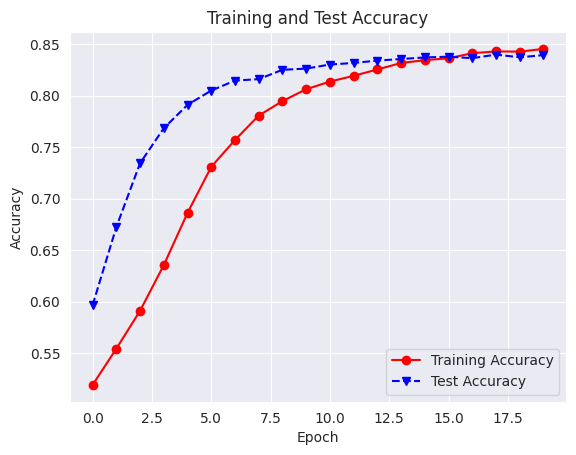
\includegraphics[width=0.50\textwidth]{mlp/Mlp_training_and_accuracy_plot}
	\caption{MLP Training and Test Accuracy Plot}\label{fig:mlp_training_and_accuracy_plot}
\end{figure}

A thorough analysis of the results reveals that the model maintains an accuracy of around 85\% throughout the epochs, indicating strong performance on the training data. In contrast, the test accuracy, though slightly lower than the training accuracy, remains stable around 80\% across epochs, suggesting reasonable generalization to unseen data. The observed gap between the training and test accuracy indicates potential overfitting, a common phenomenon where a model performs well on training data but struggles with unseen data.

\begin{figure}[H] 
	\centering
	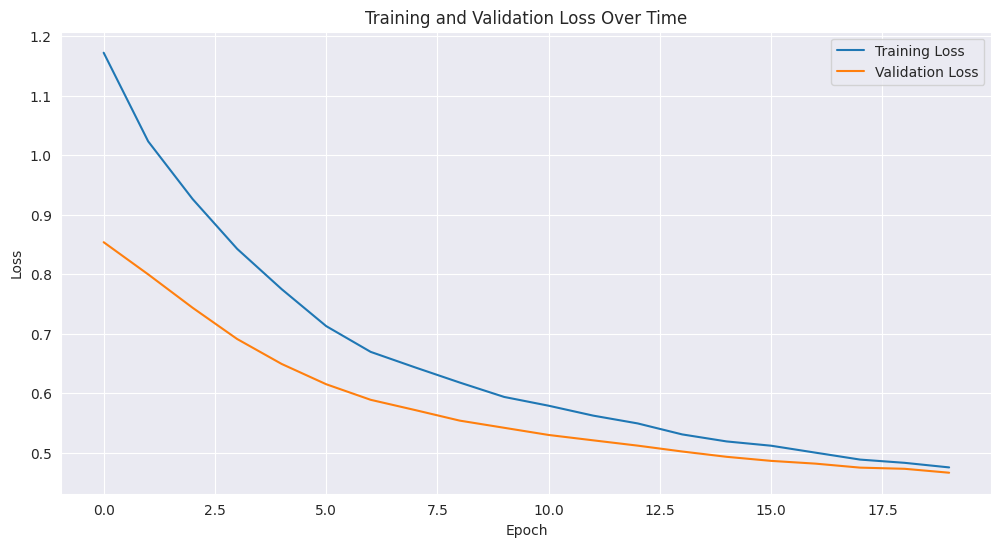
\includegraphics[width=0.50\textwidth]{mlp/Mlp_training_and_validation_loss_plot}
	\caption{MLP Training and Validation Loss Plot}\label{fig:mlp_training_and_validation_loss_plot}
\end{figure}

Additionally, the training and validation loss over time plot for this model shows a promising trend. It suggests that the model is learning effectively and avoiding overfitting. The training loss appears to be steadily decreasing over the epochs, indicating that the model is continually improving its ability to fit the training data. Similarly, the validation loss also shows a decreasing trend, although it fluctuates slightly more than the training loss. Overall, the validation loss follows a similar pattern to the training loss, indicating that the model is generalizing well and not overfitting to the training data.

\begin{figure}[H] 
	\centering
	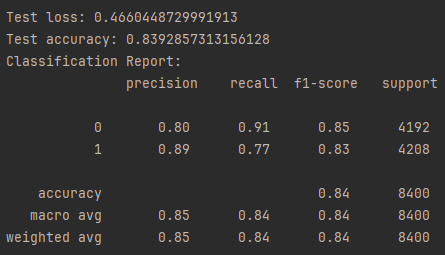
\includegraphics[width=0.50\textwidth]{mlp/Mlp_classification_report}
	\caption{Mlp Classification Report}\label{fig:mlp_classification_report}
\end{figure}

The Multilayer Perceptron (MLP) model achieved a test accuracy of 84.61\% with a test loss of 0.42. The precision for NLOS (class 0) was 81\% and for LOS (class 1) was 89\%, indicating a high level of precision in predicting both classes. The recall for NLOS was 90\% and for LOS was 79\%, showing that the model performs better at identifying NLOS instances. The F1-score, which balances precision and recall, was 85\% for NLOS and 84\% for LOS. Overall, the model demonstrates good performance in classifying NLOS and LOS instances, although there is potential for improvement in the recall for LOS to achieve a more balanced performance across both classes.

\subsubsection{Possible Improvements}

Possible improvements for the Multilayer Perceptron (MLP) model could include hyperparameter tuning, where experimenting with different hyperparameters like the number of units in Dense layers, the dropout rate, and the learning rate of the optimizer could lead to enhanced performance. Techniques such as grid search or random search can efficiently explore the hyperparameter space. Additionally, exploring more complex MLP architectures, such as adding layers or using different activation functions, may improve the model's ability to learn intricate patterns. Other regularization techniques like L1 regularization or different dropout rates could further prevent overfitting. Data augmentation methods can also be applied to increase the dataset size, potentially improving generalization. Ensemble methods, including combining MLP with other models or using bagging/boosting, could reduce variance and improve generalization. Lastly, feature engineering to identify and incorporate relevant features could enhance the model's performance by capturing underlying data patterns more effectively.

\subsubsection{Conclusion}

In conclusion, the Multilayer Perceptron (MLP) model trained for Non-Line-of-Sight (NLOS) and Line-of-Sight (LOS) classification shows strong performance, achieving an accuracy of approximately 85\%. The model demonstrates good precision and recall for both classes, indicating its effectiveness in classifying NLOS and LOS instances. However, there is room for improvement, particularly in reducing the observed gap between training and test accuracy to mitigate potential overfitting.

\subsection{Comparison Between CNN and MLP}\label{cnn_vs_mlp}

% Decide whether are you using supervised or unsupervised learning? What algorithm should be preferred for your team? %
% Decide the split ratio of the training/test dataset such as 70:30 or 80:20? %
% Determine the classification, regression performance accuracy such as RMSE, confusion matrix etc? %

% GPT4 plox @jovian%
Convolutional Neural Networks (CNNs) offer several advantages for classifying NLOS and LOS signals in UWB communication. One key advantage is their ability to automatically learn hierarchical features from the input data through convolutional and pooling layers. This feature extraction process is particularly effective for capturing complex spatial patterns in the signal data, which can be crucial for distinguishing between NLOS and LOS scenarios. Additionally, CNNs are adept at handling high-dimensional data, such as images or multi-dimensional signal data, making them well-suited for UWB signal classification tasks where the input data may have complex spatial relationships.

However, CNNs also have some limitations. They can be computationally expensive, especially when dealing with large datasets or complex network architectures. Training CNNs may require a significant amount of computational resources and time, which can be a practical limitation in some scenarios. Additionally, CNNs may be more challenging to interpret compared to simpler models like MLPs, making it harder to understand the underlying reasons for the model's predictions.

On the other hand, Multilayer Perceptrons (MLPs) have their own set of advantages and disadvantages for UWB signal classification. MLPs are relatively simpler in architecture compared to CNNs, making them easier to train and interpret. This simplicity can be advantageous in scenarios where the signal data does not have strong spatial dependencies or when computational resources are limited. MLPs are also known for their ability to learn complex relationships in data, which can be beneficial for capturing the nuances of NLOS and LOS signal characteristics.

However, MLPs may struggle with capturing spatial patterns in the signal data, especially if the data has strong spatial dependencies. Unlike CNNs, which are specifically designed for tasks involving spatial data, MLPs may not be as effective at extracting spatial features from the input data. Additionally, MLPs can be prone to overfitting, especially when dealing with high-dimensional data or complex patterns. Regularization techniques, such as dropout or L2 regularization, may be necessary to prevent overfitting in MLPs.

% \subsection{Supervised Machine Learning Algorithms}\label{sml}

% TO WRITE %


% Decide whether are you using supervised or unsupervised learning? What algorithm should be preferred for your team? %
% Decide the split ratio of the training/test dataset such as 70:30 or 80:20? %
% Determine the classification, regression performance accuracy such as RMSE, confusion matrix etc? %
\subsection{Unsupervised Machine Learning Algorithms}\label{uml}

Over the past few weeks, we explored various Unsupervised Machine Learning (UML) algorithms, each aimed at extracting meaningful insights from our dataset. Here, we provide a concise overview of the algorithms employed and the outcomes observed.

\subsubsection{Historical Data Preprocessing}

Initially, we conducted comprehensive preprocessing steps on the historical data. This included feature selection by dropping attributes with uniform values, followed by Principal Component Analysis (PCA) to transform the CIR0-1015 features into their principal components. Additionally, new features were derived using formulas sourced from the dataset's specifications.

\subsubsection{Algorithmic Trials and Observations}

The Random Forest Classifier exhibited remarkable initial accuracy, prompting further investigation into potential overfitting. Despite the promising performance, subsequent visualization revealed nuances within the model's trees, motivating us to explore alternative approaches.

Similarly, Logistic Regression demonstrated swift training but yielded perfect accuracy, raising concerns about its suitability for our dataset.

Exploring the K-Nearest Neighbors (KNN) algorithm, we conducted a grid search to determine the optimal K value. While achieving approximately 80\% accuracy, visual analysis revealed signs of overfitting, prompting us to seek alternative methods.

Naive Bayes and K-Means Clustering both showed perfect accuracy, suggesting potential overfitting. Though further exploration, such as hyperparameter tuning, could have been pursued, time constraints led us to pivot towards more informed approaches.

Support Vector Machine (SVM) also yielded perfect accuracy, prompting reflection on the need for deeper domain knowledge and additional processing techniques.

\subsubsection{Reflection and Future Directions}

Our experimentation underscored the importance of domain expertise and refined processing techniques. Recognizing the need for a deeper understanding of UWB and feature significance, we shifted our approach towards denoising methods and the application of supervised machine learning algorithms like Convolutional Neural Networks (CNN) and Multilayer Perceptrons (MLP). These techniques offer promising avenues for extracting nuanced insights from our dataset and improving classification performance.

In summary, our exploration of UML algorithms highlighted the critical role of domain knowledge and refined processing techniques in effectively analyzing complex datasets. By embracing a more informed approach, we aim to enhance the robustness and interpretability of our classification models.
